\section{Experiments}
\label{sec:exp}
We ask four questions. \textbf{Q1} Is \method's necessity map faithful? \textbf{Q2} Does one code path explain convolutional, attention and state-space models? \textbf{Q3} Is the motion/geometry split \emph{correct}? \textbf{Q4} What do its components contribute and cost?

\subsection{Setup}
\label{sec:exp-setup}
\paragraph{Data and ground truth.}
We explain action recognition on MSR-Action3D~\cite{li2010msraction3d}: 567 depth videos of 20 actions by 10 subjects, with the standard split (subjects 1--5 for training, 270 videos; 6--10 for testing, 297 videos). Depth maps become point-cloud videos with the MeteorNet protocol~\cite{liu2019meteornet} used by all three official backbones; we use centred 24-frame clips with 2048 points per frame, re-sampled independently in every frame (no point identity). MSR-Action3D also ships 20-joint skeletons. We lift them into the same coordinates, where a median \NumGTFitMedian\% of the points lie within about 12\,cm of a bone, and label every point with its nearest bone. Some videos store no skeleton for a run of frames; every ground-truth-based number leaves out the \NumGTMissing\ benchmark clips concerned. Points of bones that travel at least half as far as the clip's most active bone form the \emph{moving} ground truth (on average \NumGTMovingPct\% of a clip's points); points of bones that travel at most a fifth as far form the \emph{static} ground truth (\NumGTStaticPct\%; Appendix~\ref{supp:impl}). The main benchmark explains every test video that is at least 24 frames long (\NumPFTClips\ clips; \NumGTValid\ with a complete skeleton). The cross-backbone study, the ablations and the stability study use the first two test clips of every action (\NumCrossClips\ clips).

\paragraph{Backbones.}
We explain the \emph{unmodified official code} of the convolutional PSTNet~\cite{fan2021pstnet}, the attention-based P4Transformer~\cite{fan2021p4transformer} and the attention-free state-space Mamba4D~\cite{liu2025mamba4d}. No pretrained weights exist, so we train each from scratch at its official width on one A100 GPU, replacing the CUDA-only operators by numerically equivalent PyTorch versions (Appendix~\ref{supp:impl}). Test accuracies (video level) are \BBaccPFT/\BBaccPST/\BBaccMBA\,\% for P4Transformer/PSTNet/Mamba4D (published: 90.9/91.2/92.7). A second, laptop-scale training (reduced width, 1024 points) supports the same conclusions; Appendix~\ref{supp:scale} compares the two.

\paragraph{Baselines.}
\emph{Floors:} random; geometry-edge (local point spacing); motion prior (model-blind nearest-neighbour flow between frames). \emph{Gradient:} Grad$\times$Input, SmoothGrad~\cite{smilkov2017smoothgrad}, Integrated Gradients~\cite{sundararajan2017ig}, and 3D Grad-CAM~\cite{selvaraju2017gradcam} on the tube-embedding tokens. \emph{Perturbation:} region occlusion (deleting each tracked region, as in point-cloud saliency~\cite{zheng2019pointcloudsaliency}), OccAM~\cite{schinagl2022occam}, and extremal perturbations~\cite{fong2019extremal}. \emph{Attention (P4Transformer only):} rollout~\cite{abnar2020rollout}, transformer attribution~\cite{chefer2021transformer}, and raw attention: the attention each token receives in the last layer, used \emph{as} the explanation.
\paragraph{\method.} $m{=}12$ tracked regions; local estimator (37 passes) and context estimator ($S{=}256$, $q{=}\tfrac12$). An attribution map gives each point its region's $\Nec$; localisation uses $\Smot$ (moving GT) and $\Sgeo$ (static GT).

\paragraph{Metrics.}
\emph{Faithfulness} (no GT): deletion/insertion AUC of the target-class probability~\cite{petsiuk2018rise}, comprehensiveness/sufficiency (AOPC over $\{1,5,10,20,50\}\%$)~\cite{deyoung2020eraser}, and Sensitivity-$n$~\cite{ancona2018sensitivity}; a deleted point is removed and its frame re-sampled. \emph{Localisation} (skeleton GT): Pointing Game~\cite{zhang2018pointing} and energy-based EBPG~\cite{wang2020scorecam}. \emph{Sanity:} cascading model randomisation~\cite{adebayo2018sanity}. \emph{Statistics.} Every score is computed per clip and reported as the mean over clips. A $p$-value compares two methods on the same clips with a two-sided paired Wilcoxon signed-rank test~\cite{wilcoxon1945}; $p$-values in the text are uncorrected, and a $^\ast$ in a table marks \method\ better than the strongest baseline after Bonferroni correction over that table's metrics~\cite{dunn1961}. Intervals are 95\% percentile bootstrap intervals over clips (2000 resamples)~\cite{efron1979bootstrap}. Appendix~\ref{supp:provenance} lists the data, models and code behind every table and figure.


\begin{table*}[t]
\centering\small\tablecitesoff
\begin{tabular}{l cccc}
\toprule
Method & Del.$\downarrow$ & Comp.$\uparrow$ & Ins.$\uparrow^\dagger$ & Suff.$\downarrow^\dagger$\\
\midrule
\tabinput{tables/tab_faithfulness.tex}
\bottomrule
\end{tabular}
\caption{\textbf{Faithfulness} on P4Transformer, MSR-Action3D test set (all \NumPFTClips\ test clips; mean$\pm$std over clips). Del.: deletion AUC of the target-class probability; Comp.: comprehensiveness. Both remove the top-ranked points. Ins.\ and Suff.\ ($\dagger$) \emph{keep} the top-ranked points, which rewards spatially scattered rankings on point clouds (a random subset preserves the whole body; see the random floor). \textbf{Bold}: best, \underline{underlined}: second, floors excluded. $^\ast$: \method\ significantly better than the strongest baseline after Bonferroni correction.}
\label{tab:faithfulness}
\end{table*}

\subsection{Faithfulness (Q1)}
\label{sec:exp-main}
Tab.~\ref{tab:faithfulness} and Fig.~\ref{fig:curves} compare the necessity maps. \method's context estimator attains the lowest deletion AUC (\NumPFTKcaCtxDel; local estimator \NumPFTKcaDel) and the highest comprehensiveness. Its deletion AUC is significantly below that of region occlusion (\NumPFTOcclDel; paired Wilcoxon $p\NumPKcaCtxOcclDel$) and of Integrated Gradients (\NumPFTIGDel; $p\NumPKcaCtxIGDel$), and far ahead of attention rollout (\NumPFTRolloutDel), transformer attribution (\NumPFTTAttrDel) and raw attention (\NumPFTSTAADel): on the very backbone that has attention, reading it out is a poor explanation. Two findings deserve comment. \emph{(i) Region occlusion is \method's necessity with a deletion corner.} Replacing the static proxy of Sec.~\ref{sec:method-interventions} by deletion makes the local necessity map \emph{identical} to region occlusion, which the deletion metric (itself deletion-based) favours over the local estimator ($p\NumPKcaOcclDel$); the context estimator more than recovers the gap, and the proxy is what makes the motion/geometry split meaningful (Sec.~\ref{sec:exp-mpg}, Tab.~\ref{tab:ablation}). \emph{(ii) Point-cloud models shrug off random point dropout.} Deleting points in random order leaves the prediction almost intact (Fig.~\ref{fig:curves}), so point-level random masking (OccAM, \NumPFTOccamDel) and soft-mask optimisation (Extremal, \NumPFTExtremalDel) carry little signal at this budget, and \emph{keep}-based metrics reward scattered rankings: the random floor scores an insertion AUC of \NumPFTRandomIns. We therefore read faithfulness mainly from the deletion-based columns.

\begin{figure*}[t]
\centering
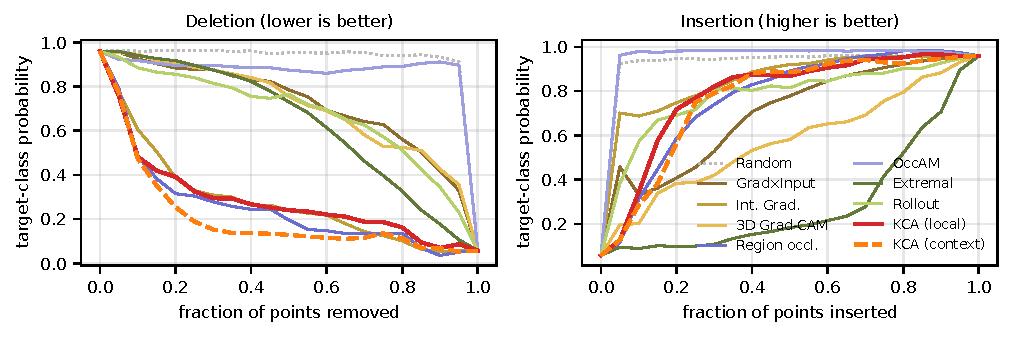
\includegraphics[width=\textwidth]{fig/msr_curves.pdf}
\caption{\textbf{Deletion and insertion curves} on P4Transformer (mean over the \NumPFTClips\ clips of Tab.~\ref{tab:faithfulness}): target-class probability vs.\ fraction of points removed (left) or inserted (right), in 20 steps.}
\label{fig:curves}
\end{figure*}

\begin{table*}[t]
\centering\small\tablecitesoff
\begin{tabular}{l cc cc cc}
\toprule
& \multicolumn{2}{c}{PSTNet} & \multicolumn{2}{c}{P4Transformer} & \multicolumn{2}{c}{Mamba4D}\\
\cmidrule(lr){2-3}\cmidrule(lr){4-5}\cmidrule(lr){6-7}
Method & Del.$\downarrow$ & EBPG$\uparrow$ & Del.$\downarrow$ & EBPG$\uparrow$ & Del.$\downarrow$ & EBPG$\uparrow$\\
\midrule
\tabinput{tables/tab_cross.tex}
\bottomrule
\end{tabular}
\caption{\textbf{Across backbones} (the same \NumCrossClips\ test clips, two per action, for every backbone; means over clips): deletion AUC and localisation of the moving ground truth (EBPG, on the clips with a complete skeleton; $\Smot$ for \method). Attention methods are undefined on PSTNet and Mamba4D (n/a). Kendall's $\tau$~\cite{kendall1938} between the rankings by Del.\ of the 7 methods defined on all three backbones: PSTNet--P4Transf.\ \NumTauPSTPFT, PSTNet--Mamba4D \NumTauPSTMBA, P4Transf.--Mamba4D \NumTauPFTMBA.}
\label{tab:cross}
\end{table*}

\subsection{Across backbones (Q2)}
\label{sec:exp-cross}
Tab.~\ref{tab:cross} runs the same code on the three official architectures. \method is defined on all of them---the attention methods are not. On every backbone its context estimator has the lowest or second-lowest deletion AUC, statistically tied with region occlusion on PSTNet and Mamba4D (paired Wilcoxon $p\NumPPSTKcaCtxOcclDel$, $p\NumPMBAKcaCtxOcclDel$) and below Integrated Gradients, significantly on PSTNet ($p\NumPPSTKcaCtxIGDel$) but not on Mamba4D ($p\NumPMBAKcaCtxIGDel$); its motion term localises the moving parts on par with Integrated Gradients, the best single map ($p\NumPPSTKcaCtxIGEBPG$, $p\NumPMBAKcaCtxIGEBPG$), and at least as well as region occlusion. The method ranking is consistent across backbones (Kendall $\tau$, caption), and the state-space Mamba4D, which has no attention to read, is explained exactly like the others. On PSTNet and Mamba4D every informative map puts less mass on the moving parts than on P4Transformer: these models spread their evidence more widely (Sec.~\ref{sec:exp-qual}).

\begin{table}[t]
\centering\small\tablecitesoff\setlength{\tabcolsep}{3pt}
\begin{tabular}{l cc c cc}
\toprule
& \multicolumn{2}{c}{$\to$ moving GT} & $\to$ static & \multicolumn{2}{c}{crossover: cue =}\\
\cmidrule(lr){2-3}\cmidrule(lr){4-4}\cmidrule(lr){5-6}
Method & PG$\uparrow$ & EBPG$\uparrow$ & PG$\uparrow$ & motion & shape\\
\midrule
\tabinput{tables/tab_localization.tex}
\bottomrule
\end{tabular}
\caption{\textbf{Motion vs.\ geometry} (P4Transformer). Left: localisation against the skeleton ground truth on the \NumGTValid\ clips of Tab.~\ref{tab:faithfulness} with a complete skeleton (PG: Pointing Game; $\Smot$ against moving, $\Sgeo$ against static parts). Right: \emph{crossover} (Sec.~\ref{sec:exp-mpg}, \NumXEval\ test clips per task), motion share $\Smot^+/(\Smot^++\Sgeo^+)$ of the positive importance on the arm; single maps have no split (--).}
\label{tab:mpg}
\end{table}

\subsection{Motion versus geometry (Q3)}
\label{sec:exp-mpg}
\paragraph{Localisation.} $\Smot$ places \NumPFTKcaCtxSmotEBPG\ of its positive mass on the skeleton's moving parts (EBPG, Tab.~\ref{tab:mpg}), above region occlusion (\NumPFTOcclEBPG) and far above the model-blind motion prior (\NumPFTMotionPriorEBPG), whose mass is spread over sensor jitter, but below the best single map, Integrated Gradients (\NumPFTIGEBPG; $p\NumPKcaCtxIGEBPG$). The single most-salient point of Integrated Gradients hits the moving parts more often (PG), since region-constant maps have no ranking \emph{within} a region. On moving parts, \NumPFTKcaCtxMotShareMoving\ of \method's positive importance is motion, against \NumPFTKcaCtxMotShareAll\ over the whole body. Localisation, however, is confounded: moving parts are also geometrically distinctive, so a map that highlights the arm for \emph{any} reason scores well.
\paragraph{Crossover: the decisive test.} We therefore build two binary tasks from real clips in which the classes differ \emph{only} in the right arm: in the \emph{motion} task one class replays the arm at $25\%$ speed (its shape is real), in the \emph{shape} task one class thickens the arm $3\times$ about its bones (its motion is untouched). We keep the videos in which the right arm carries at least 30\% of the skeleton's motion (\NumXTrain\ training and \NumXTest\ test videos, one centred clip each) and train one P4Transformer per task; its accuracy over both classes of the test clips is \NumXMotAcc\ / \NumXGeoAcc\,\% (motion / shape task). In each task we explain the class whose defining property is present and removable by the interventions---normal-speed motion (removed by \frz) and the thick shape (removed by the proxy). We explain the first \NumXEval\ test clips and pool the positive $\Smot$ and $\Sgeo$ over their arm points. For the \emph{same} arm, the motion share of \method's importance is \NumXMotShare\ for the motion model (95\% bootstrap CI [\NumXMotLo, \NumXMotHi]; context estimator \NumXMotShareCtx) and \NumXGeoShare\ for the shape model ([\NumXGeoLo, \NumXGeoHi]; context \NumXGeoShareCtx)---a gap of [\NumXGapLo, \NumXGapHi]---whereas the model-blind motion prior marks the arm identically in both tasks (EBPG \NumXMotPriorEBPG\ vs.\ \NumXGeoPriorEBPG). Across \NumXSeedsTotal\ training seeds of the two task models, the motion-task model leaves chance in only \NumXSeedsTrained; in all \NumXSeedsSameDir\ of these the arm's motion share is higher in the motion task, with an interval that excludes zero in \NumXSeedsCIExcl\ (Tab.~\ref{tab:seeds}). The split is not all-or-nothing on real models---the shape model still reacts to freezing the arm, whose frozen pose changes its per-frame configuration---but it moves with the cue, which no single map can show. Repeating the test with the convolutional PSTNet (\NumXPstMotAcc\ / \NumXPstGeoAcc\,\% accuracy) gives a cleaner split, \NumXPstMotShare\ vs.\ \NumXPstGeoShare\ (gap [\NumXPstGapLo, \NumXPstGapHi]), and the state-space Mamba4D (\NumXMbaMotAcc\ / \NumXMbaGeoAcc\,\%) one similar to P4Transformer, \NumXMbaMotShare\ vs.\ \NumXMbaGeoShare\ (gap [\NumXMbaGapLo, \NumXMbaGapHi]). On these two backbones the shape model still draws more than half of the arm's importance from motion, in line with their motion-heavy maps on MSR (whole-body motion share \NumMBAKcaCtxMotShareAll\ for Mamba4D, \NumPFTKcaCtxMotShareAll\ for P4Transformer): the audit shows which cue a model responds to, not that it uses that cue alone. Fig.~\ref{fig:dissoc} summarises all three next to the fully controlled setting of Appendix~\ref{supp:controlled} (\NumCtrlMot\ vs.\ \NumCtrlShape).

\begin{figure}[t]
\centering
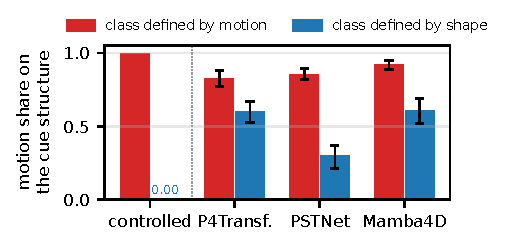
\includegraphics[width=0.9\linewidth]{fig/dissociation.pdf}
\caption{\textbf{Double dissociation:} motion share on the cue structure when the class is defined by its motion (red) or by its shape (blue), local estimator. Controlled task: pooled over 3 seeds $\times$ 20 clips. Real crossover: \NumXEval\ test clips per task and backbone, with 95\% bootstrap intervals.}
\label{fig:dissoc}
\end{figure}


\subsection{Ablation, sanity and cost (Q4)}
\label{sec:exp-ablation}
\paragraph{Components (Tab.~\ref{tab:ablation} in the appendix).} \emph{Redundancy:} with a fine partition ($m{=}24$) a body part spans several regions and the local necessity collapses (deletion AUC \NumAblLocalFineDel), while the context estimator keeps it (\NumAblCtxFineDel)---the failure mode it was designed for. \emph{The $(0,0)$ corner:} deleting the region instead of using the static proxy aligns the necessity with the deletion metric (local \NumAblLocalDel$\to$\NumAblLocalBgDel; context \NumAblCtxDel$\to$\NumAblCtxBgDel, the best of all variants) but weakens the motion term's localisation (EBPG \NumAblLocalEBPG$\to$\NumAblLocalBgEBPG); in the controlled study, where the answer is known, the same change makes a pure-shape model look \NumCtrlBgShape\% motion-driven (Appendix~\ref{supp:controlled}). \emph{The order:} the motion-first scores absorb the interaction into $\Smot$ (motion share \NumAblLocalMotionFirstShare\ vs.\ \NumAblLocalShare\ symmetric). $S{=}64$ samples already give \NumAblCtxSsixtyfourDel\ (vs.\ \NumAblCtxDel\ at $S{=}256$). Anchoring \frz\ and the proxy at the middle instead of the first frame barely changes the split (motion share \NumAblLocalMidShare\ vs.\ \NumAblLocalShare) and does not hurt faithfulness (Tab.~\ref{tab:ablation}). The interaction is \emph{not} negligible on real models ($|\Delta_{\mathrm{int}}|/|\Nec|$ in the table, against \NumCtrlProxyDint\ for the controlled network), which is exactly why we report order-symmetric scores and the residual rather than assume separability.
\paragraph{Sanity.} Under the cascading randomisation of \citet{adebayo2018sanity}, applied to P4Transformer from the head down on 20 clips (Fig.~\ref{fig:sanity} in the appendix), the rank correlation of \method's map with the trained model's drops to \NumSanHeadKca\ as soon as the head is re-initialised and stays within $\pm0.2$ (\NumSanKca\ with every block randomised): the explanation depends on the learned weights. Grad$\times$Input keeps a correlation of \NumSanGxI\ even then---much of it reflects the input rather than the model. On the region with the largest $\Smot$ (\NumCrossClips\ clips), freezing it changes the prediction in \NumDspFreezeFlip\% of the clips and reversing its trajectory (\dsp) in \NumDspReverseFlip\%: most motion evidence is about \emph{whether} a part moves, less about \emph{which way}.

\paragraph{Stability under re-sampling.} A sensor never returns the same points twice, so we re-sample each of the \NumCrossClips\ clips \NumStabSamplings\ times, explain every sampling, map each explanation onto the points of the first one and rank-correlate the two (Tab.~\ref{tab:stability} in the appendix). The prediction stays the same in \NumStabPredSame\% of the samplings. \method's maps are the less stable ones point by point: \NumStabKcaCtxPoint\ for the context estimator against \NumStabIGPoint\ for Integrated Gradients and \NumStabOcclPoint\ for region occlusion, because the regions are re-fitted to every sampling. At the level of body parts (each map averaged over the 19 skeleton bones) the gap narrows (\NumStabKcaCtxPart\ vs.\ \NumStabIGPart), and the whole-body motion share varies little between samplings (standard deviation \NumStabKcaCtxShareSD). Averaging the maps of two samplings, which costs only forward passes, raises the context estimator to \NumStabKcaCtxAvgPoint\ (points) and \NumStabKcaCtxAvgPart\ (parts).

\paragraph{Cost.} On one A100 GPU (mean over the \NumPFTClips\ clips), the local estimator takes \NumPFTKcaTime\,s per clip and the context estimator \NumPFTKcaCtxTime\,s ($S{=}256$ random states, batched), comparable to OccAM (\NumPFTOccamTime\,s) and Integrated Gradients (\NumPFTIGTime\,s). All passes are independent forward queries, so the cost falls with batch throughput and needs no backward pass.

\subsection{Qualitative results}
\label{sec:exp-qual}
Fig.~\ref{fig:teaser} and Fig.~\ref{fig:qual} in the appendix overlay $\Smot$ and $\Sgeo$ on real test clips. On \emph{draw circle} all three backbones put their strongest motion importance on the drawing hand, and on \emph{forward kick} P4Transformer and PSTNet put it on the kicking leg. \emph{High arm wave} is different: PSTNet marks the raised hand, but P4Transformer and Mamba4D put their motion importance on the torso rather than on the waving arm. Geometry importance spreads more widely over the body on every backbone. Per-action statistics are in Tab.~\ref{tab:per-class}.
